\usetikzlibrary{positioning, calc}
\chapter{graficos2}

	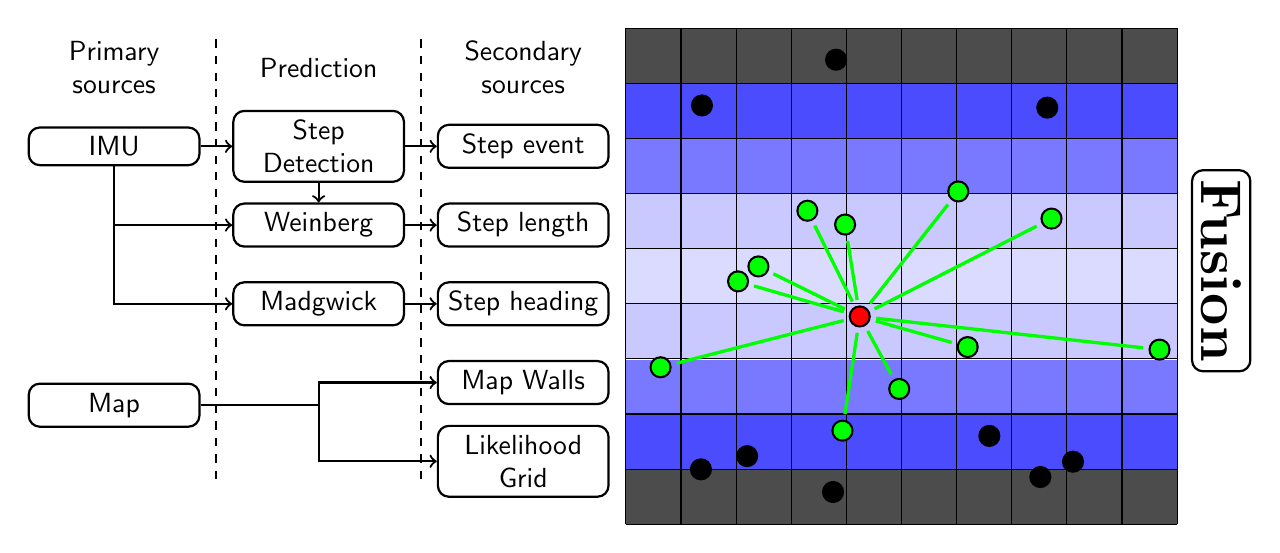
\begin{tikzpicture}[
		dot/.style = {circle, minimum size= 8,fill,inner sep=0pt, outer sep=0pt},
		dot/.default = 5pt
		]
		% Drawing the likelihood grid
		% Horizontal cells count
		\def\lowbound{0}
		\def\highbound{9}
		
		\begin{scope}[shift={(0,0.5)}, scale=0.7]
			\tikzstyle{cell} = [rectangle, minimum size = 19.5 , fill, color = black]
			\draw [black, step = 1] (\lowbound, 1) grid (\highbound+1, 10);
			
			\begin{scope}[shift = {(0.5,0.5)}, opacity = 0.7]
				\foreach \x in {\lowbound,1,...,\highbound}{
					\node [cell, black] at  (\x, 9) {};
					\node [cell, black] at  (\x, 1) {};
				} % black cells = walls
				\foreach \x in {\lowbound, 1,..., \highbound}{
					\node [cell, color = blue!100!white] at  (\x, 8) {};
					\node [cell, color = blue!100!white] at  (\x, 2) {};
				} % deep blue cells
				\foreach \x in {\lowbound,1,...,\highbound}{
					\node [cell, color = blue!75!white] at  (\x, 7) {};
					\node [cell, color = blue!75!white] at  (\x, 3) {};
				}         
				\foreach \x in {\lowbound,1,...,\highbound}{
					\node [cell, color = blue!30!white] at  (\x, 6){};
					\node [cell, color = blue!30!white] at  (\x, 4){};
				}        
				\foreach \x in {\lowbound,1,...,\highbound}{
					\node [cell, color = blue!20!white] at  (\x, 5){};
				}
			\end{scope}
			% Adding particles with random numbers drawn from a python script
			% Yes, LaTeX/Tikz allow to draw random numbers but these come from an experiment
			\begin{scope}
				\coordinate [dot] (a) at (3.9285231, 2.6985591);
				\coordinate [dot] (b) at (1.3611608, 1.9969122);
				\coordinate [dot] (c) at (0.6288356, 3.84908  );
				\coordinate [dot] (e) at (9.6810041, 4.1691515);
				\coordinate [dot] (f) at (7.644834 , 8.55942  );
				\coordinate [dot] (g) at (6.0297038, 7.0389246);
				\coordinate [dot] (h) at (3.2925639, 6.6886047);
				\coordinate [dot] (i) at (1.3797099, 8.5992524);
				\coordinate [dot] (j) at (8.1116873, 2.1354121);
				\coordinate [dot] (k) at (7.7211166, 6.5463598);
				\coordinate [dot] (l) at (6.5935806, 2.6034567);
				\coordinate [dot] (m) at (3.9761724, 6.4383623);
				\coordinate [dot] (n) at (2.4039057, 5.6784096);
				\coordinate [dot] (o) at (4.9582929, 3.4551362);
				\coordinate [dot] (p) at (3.7579452, 1.5857479);
				\coordinate [dot] (q) at (6.2010185, 4.215724 );
				\coordinate [dot] (r) at (2.0341973, 5.4074832);
				\coordinate [dot] (s) at (3.8130486, 9.4286342);
				\coordinate [dot] (t) at (7.518949 , 1.857585 );
				\coordinate [dot] (u) at (2.1995326, 2.236611 );
			\end{scope}
			
			% circle on top of each coordinate
			\foreach \i in {a,c,e,k,n,r,m,o,q,h,g}
			\draw [green, fill] (\i) circle [radius = 0.15];
			
			% draw the conenction to the green particles
			\coordinate [dot] (mean) at (4.2424450, 4.7708627);
			\draw [red, fill] (mean) circle [radius = 0.15];
			\draw (mean) edge 
			[stroke=black, very thick, green, shorten <=2, shorten >=2] (a);
			\draw (mean) edge 
			[stroke, very thick, green, shorten <=2, shorten >=2] (c);
			\draw [stroke, very thick, green, shorten <=2, shorten >=2]
			(mean) -- (e);
			
			% shorten allows to cut the edge before reaching a node
			\foreach \i in {k,n,r,m,o,q,h,g}
			\draw (mean) edge [very thick, green, shorten <=2, shorten >=2] (\i);
			
			\begin{scope}[shift={(10.8,5.6)}]
				\node [rotate=-90,
				thick,
				rectangle, 
				rounded corners, 
				draw,
				text width=, 
				minimum height=15,
				align = center](fusion) {\huge\textbf{Fusion}};
			\end{scope}
		\end{scope}
		
		\begin{scope}[
			shift={(-6.5,7)},
			scale=1, font = {\sffamily},
			every path/.style = {thick},
			every node/.style = {
				thick,
				rectangle, 
				rounded corners, 
				draw,
				text width = 55, 
				minimum height = 12,
				align=center
			},
			empty/.style={color = white, text= black},
			void/.style={fill = white, minimum size = 0}
			]
			
			% This is one way to define space between blocs:
			\def\hspacer{0.5} % spacing between columns
			\def\vspacer{1} % spacing between lines
			
			%%%%%%% Acquisition
			\node[empty] (input) {Primary sources};
			\node[below of = input] (imu) {IMU};
			\node[below of = imu, below = 2*\vspacer] (map) {Map};
			\coordinate [below of = map] (dots);
			
			%%%%%%%% Prediction
			\node[right of = input, right = \hspacer, empty] (prediction) {Prediction};
			\node[below of = prediction] (detect) {Step Detection};
			\node[below of = detect] (weinberg) {Weinberg};
			\node[below of = weinberg] (madgwick) {Madgwick};
			
			%%%%%%%%% Output
			\node[right of = prediction, right = \hspacer, empty] (output)
			{Secondary sources};
			\node[below of = output] (events) {Step event};
			\node[below of = events] (lengths) {Step length};
			\node[below of = lengths] (angles) {Step heading};
			
			\node[below of = angles] (walls) {Map Walls};
			\node[below of = walls] (grid) {Likelihood Grid};
			
			%% Links
			\draw [->] (imu)--(detect);
			\draw [->] (imu)|-(weinberg);
			%
			\draw [->] (imu)|-(madgwick);
			%
			\draw [->] (detect)--(events);
			\draw [->] (weinberg)--(lengths);
			\draw [->] (detect)--(weinberg);
			%
			\draw [->] (madgwick)--(angles);
			%
			\draw [->] (map.east)  -| ($(map)!0.5!(walls)$) coordinate |-(walls);
			\draw [->] (map)       -| ($(map)!0.5!(walls)$)            |-(grid);
			%
			
			% Draw columns sperators
			
			\draw [dashed] ($(input.north)     !0.5!(prediction.north)$) 
			--($(input)     !0.5!(prediction)+(dots.south)$);
			\draw [dashed] ($(prediction.north)!0.5!(output.north)$)     
			--($(prediction)!0.5!(output)    +(dots.south)$);
		\end{scope}
	\end{tikzpicture}